\begin{frame}{FlowChart (1/2)}

Already processes all possible alignments in the foldrec file. Threading
is computed on all the templates (not only one) and the DOPE score is
calculated for each couple template/threading.

\end{frame}

\begin{frame}{FlowChart (2/2)}

\begin{figure}
\centering
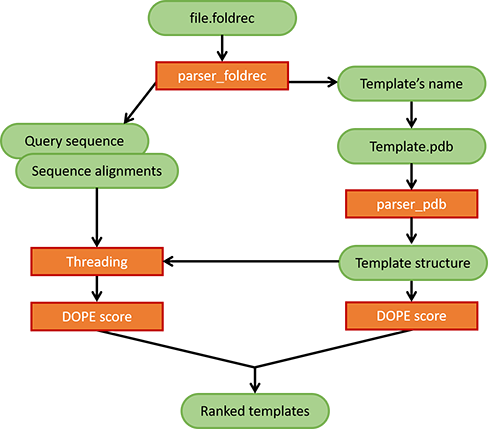
\includegraphics{FlowChart.png}
\caption{FlowChart}
\end{figure}

\end{frame}

\begin{frame}[fragile]{Data structure (1/2)}

Dictionaries of dictionaries wrapped with class objects for easier
handeling

Example of class:

\begin{Shaded}
\begin{Highlighting}[]
\KeywordTok{def} \FunctionTok{__init__}\NormalTok{(}
            \VariableTok{self}\NormalTok{: }\StringTok{'Atom'}\NormalTok{,}
\NormalTok{            x: }\BuiltInTok{float}\NormalTok{, y: }\BuiltInTok{float}\NormalTok{, z: }\BuiltInTok{float}\NormalTok{,}
\NormalTok{            element: }\BuiltInTok{str}\NormalTok{,}
\NormalTok{            atom_num: }\BuiltInTok{int}\NormalTok{,}
\NormalTok{            ) }\OperatorTok{->} \VariableTok{None}\NormalTok{:}
    \VariableTok{self}\NormalTok{.coord }\OperatorTok{=}\NormalTok{ np.array([x, y, z])}
    \VariableTok{self}\NormalTok{.element }\OperatorTok{=}\NormalTok{ element}
    \VariableTok{self}\NormalTok{.atom_num }\OperatorTok{=}\NormalTok{ atom_num}
\end{Highlighting}
\end{Shaded}

\end{frame}

\begin{frame}[fragile]{Data structure (2/2)}

Example of functions defined in the object:

\begin{Shaded}
\begin{Highlighting}[]
\KeywordTok{def}\NormalTok{ get_seq(}\VariableTok{self}\NormalTok{: }\StringTok{'Chain'}\NormalTok{):}
    \CommentTok{"""}
\CommentTok{    Return chain sequence as a string of 1 letter coded AA.}
\CommentTok{    """}
\NormalTok{    seq }\OperatorTok{=} \BuiltInTok{str}\NormalTok{()}
    \ControlFlowTok{for}\NormalTok{ res }\KeywordTok{in} \VariableTok{self}\NormalTok{.residues.values():}
        \ControlFlowTok{try}\NormalTok{:}
\NormalTok{            seq }\OperatorTok{+=}\NormalTok{ three2one[res.res_name]}
        \ControlFlowTok{except} \PreprocessorTok{KeyError}\NormalTok{:}
\NormalTok{            seq }\OperatorTok{+=} \StringTok{'X'}
    \ControlFlowTok{return}\NormalTok{ seq}
\end{Highlighting}
\end{Shaded}

=\textgreater{} class function make things faster (Antoine's argument)

\end{frame}

\begin{frame}[fragile]{Parsing foldrec and sequence threading}

\texttt{.foldrec} files are parsed and return a dictionary that can be
easily used for threading:
\texttt{\{align\_struct:\ list\ of\ tupes\ (query\ residue\ name,\ template\ residue\ number)\}}

\end{frame}

\begin{frame}{Threading of query's CA on template's CA}

Threading of query's CA on template's CA. Writes a pdb file that we can
open with PyMol.

\emph{Il serait bien de le montrer et d'avoir une image pymol ici.}

\end{frame}

\begin{frame}{DOPE score}

Sum of statistical potentials between pairs of residues (CA of residues
only for now).

Calculated on template and query =\textgreater{} Using a ``ratio'' to
compare the increase of the score from Template to threading and choose
the best template(s), i.e.~smallest decrease.

\end{frame}

\begin{frame}{Technical goals}

\begin{block}{Fast computing and execution}

Partially fulfilled: dedicated class objects, mostly working with
dictionaries (protein strutures, dope.par), limited number of lists and
iterations

\end{block}

\begin{block}{Reliable (Accurate, error free, readable)}

Partially fulfilled: Circle CI, pytest, Yvan

\end{block}

\begin{block}{Flexible (adapted to several situations)}

Partially fulfilled: pdb parser ran on all homery.foldrec templates, MSE
residue exeption handled, etc.

\end{block}

\end{frame}

\begin{frame}{Conclusion}

\begin{block}{Short term improvements}

Re-weighting DOPE scores(Sequence coverage, gaps in query, etc.)

\end{block}

\begin{block}{Long term improvements}

We want to implement the largest number of promising methods to get
several scores and find a final score using ML methods that best predict
the closest template.

\end{block}

\end{frame}
